\documentclass{article}

\usepackage{arxiv}
\usepackage[utf8]{inputenc} % allow utf-8 input
\usepackage[T1]{fontenc}    % use 8-bit T1 fonts
\usepackage{hyperref}       % hyperlinks
\usepackage{url}            % simple URL typesetting
\usepackage{booktabs}       % professional-quality tables
\usepackage{amsfonts}       % blackboard math symbols
\usepackage{nicefrac}       % compact symbols for 1/2, etc.
\usepackage{microtype}      % microtypography
\usepackage{cleveref}       % smart cross-referencing
\usepackage{lipsum}         % Can be removed after putting your text content
\usepackage{graphicx}
\usepackage{natbib}
\usepackage{doi}
\usepackage{listings}

\title{Colonies - Compute Continuums across Platforms}

\author{{\hspace{1mm}Johan Kristiansson} \\
	Department of Computer Science \\
	RISE Research Institutes of Sweden \\
	Luleå, Sweden \\
	\texttt{johan.kristiansson@ri.se} \\
	\And
	{\hspace{1mm}Thomas Ohlson Timoudas} \\
	Department of Computer Science \\
	RISE Research Institutes of Sweden \\
	Luleå, Sweden \\
	\texttt{thomas.ohlson.timoudas@ri.se} \\
	\And
	{\hspace{1mm}Henrik Forsgren} \\
	Department of Computer Science \\
	RISE Research Institutes of Sweden \\
	Luleå, Sweden \\
	\texttt{thomas.ohlson.timoudas@ri.se} \\
}

% Uncomment to override  the `A preprint' in the header
%\renewcommand{\headeright}{Technical Report}
%\renewcommand{\undertitle}{Technical Report}
\renewcommand{\shorttitle}{\textit{arXiv} Template}

%%% Add PDF metadata to help others organize their library
%%% Once the PDF is generated, you can check the metadata with
%%% $ pdfinfo template.pdf
\hypersetup{
pdftitle={A template for the arxiv style},
pdfsubject={q-bio.NC, q-bio.QM},
pdfauthor={David S.~Hippocampus, Elias D.~Striatum},
pdfkeywords={First keyword, Second keyword, More},
}

\begin{document}
\maketitle

\begin{abstract}
Running AI/ML models in production is becoming more widespread, and maintaining these systems is more complex 

    This paper presents a novel framework for managing computational workload across heterogeneous platforms. Colonies is based on  
a loosly coupled microservice architecture where complex workflows are broken down in composable functions that are executed by independently deployable executors. Using a HTTP protocol, workflows can be expressed declarative in any computer language and be executed across platforms by so-called executors, independently deployed in the cloud, edge, devices, or even in web browser creating compute continuums across platforms. Colonies supports both real-time processing and batch jobs while at the same time offer full tracability and zero-trust security.  

The paper 

\end{abstract}

% keywords can be removed
\keywords{Serverless computing \and Parallel computing \and Workflow orchestration}

\section{Introduction}
TODO
https://modelserving.com/blog/why-do-people-say-its-so-hard-to-deploy-a-ml-model-to-production
\section{The Colonies framework}
\label{sec:headings}

\subsection{Architecture}
TODO
\begin{figure}[h]
	\centering
    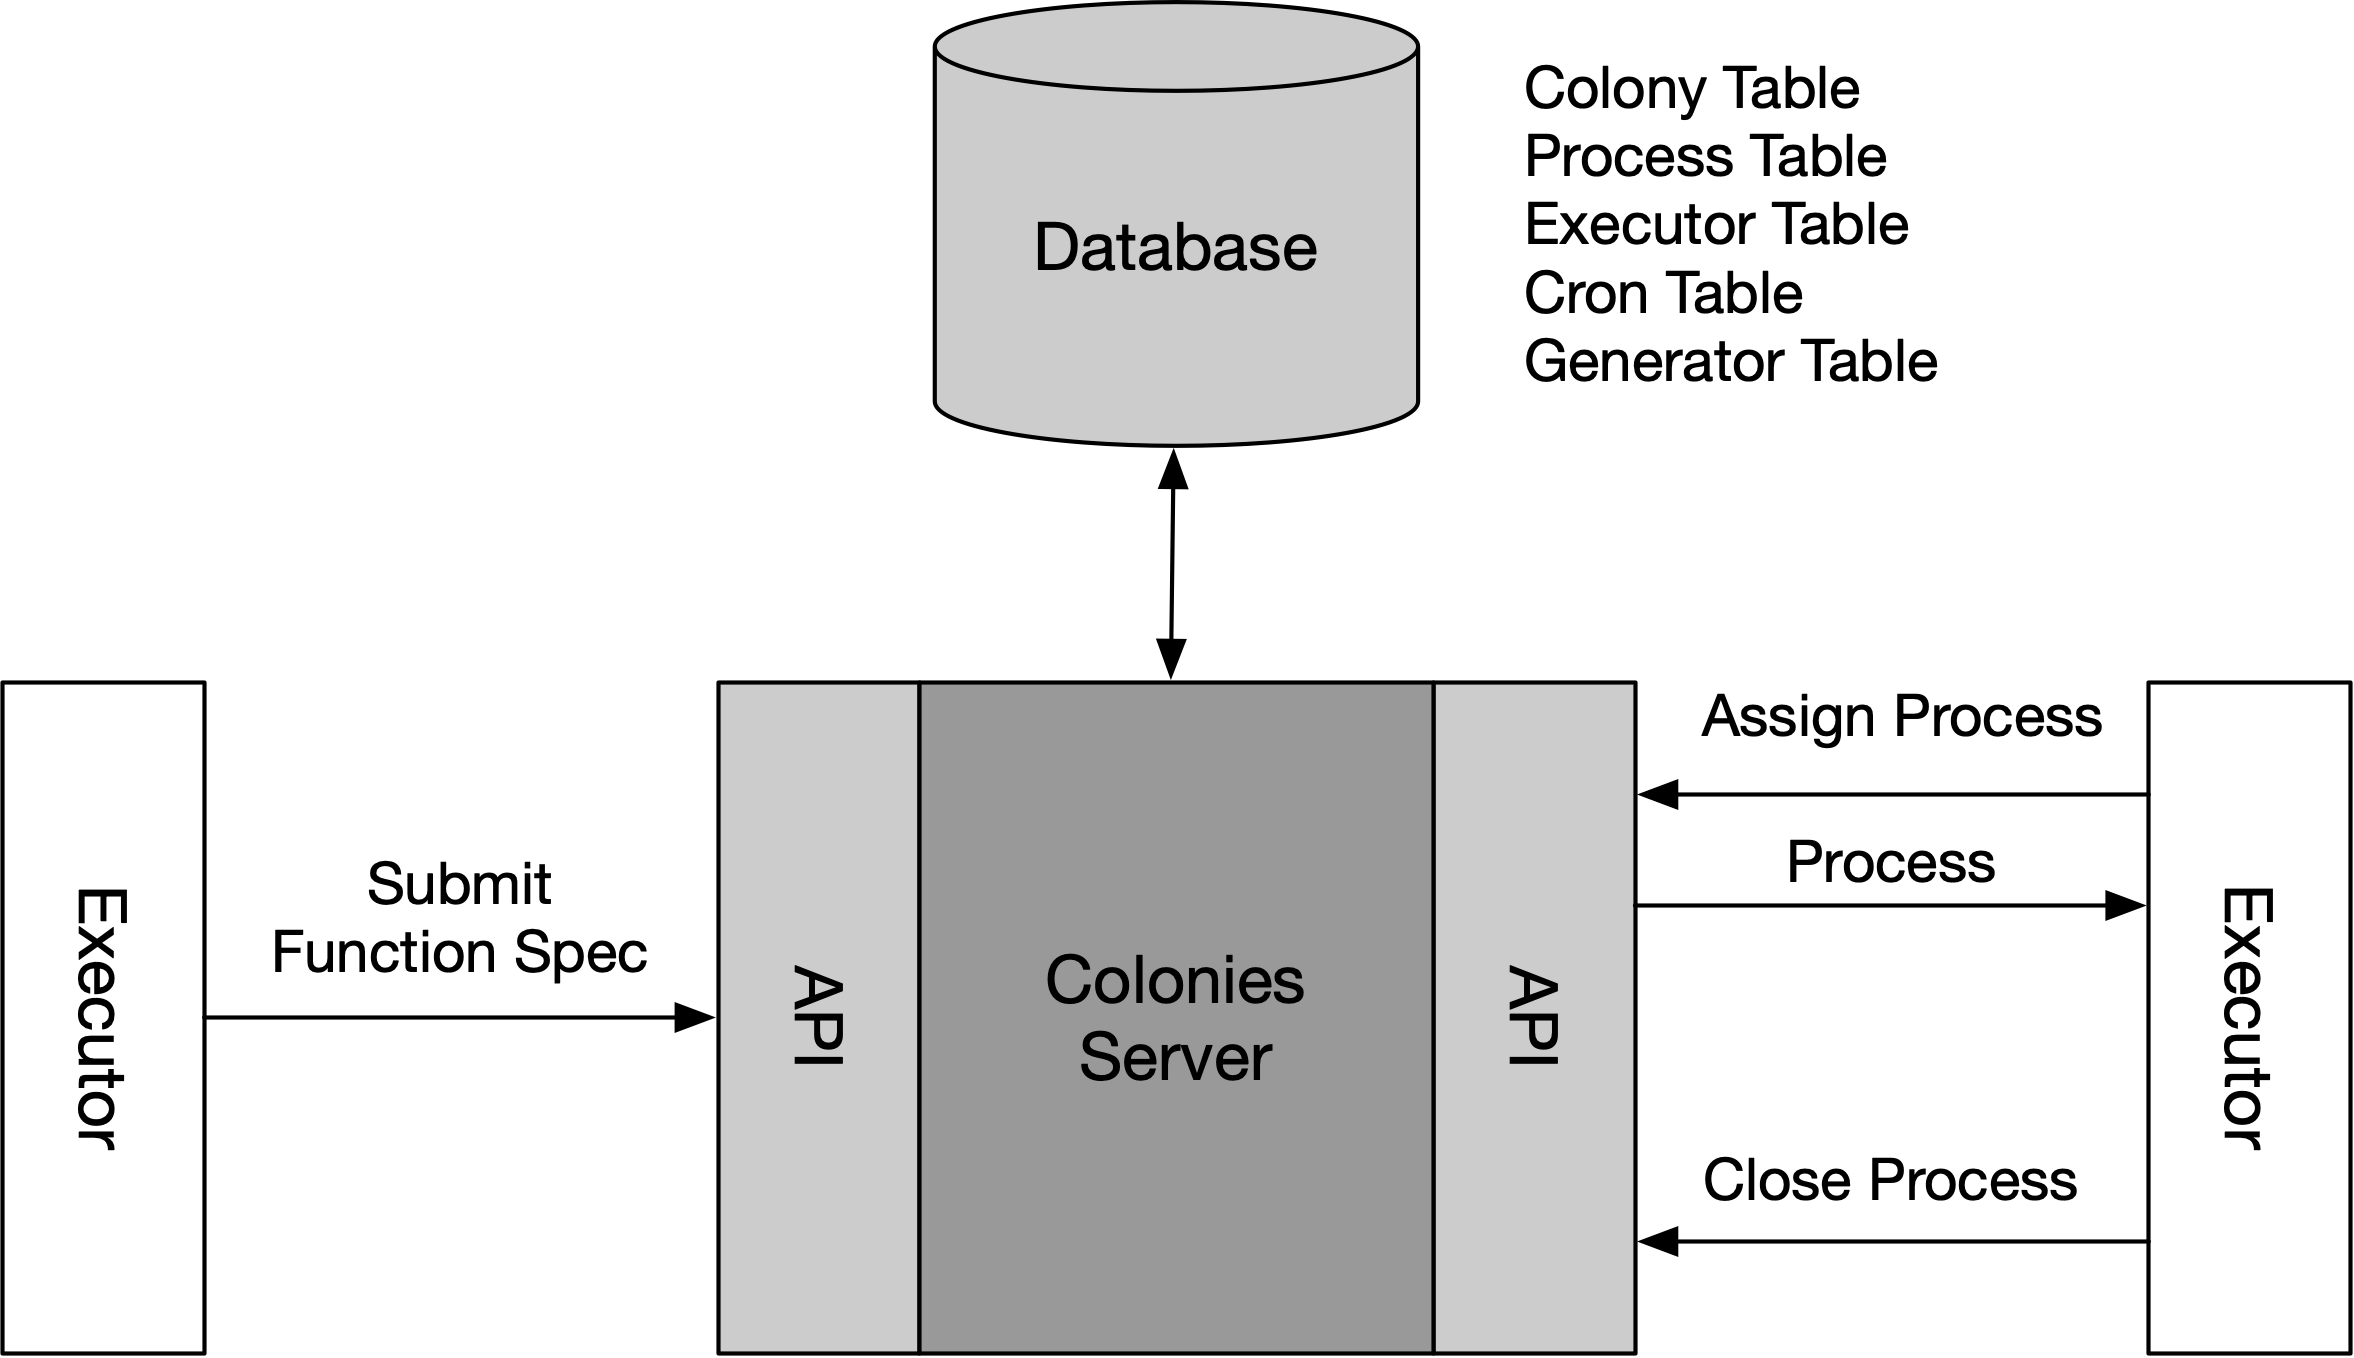
\includegraphics[scale=0.4]{arch.png}
	\caption{cron management}
	\label{fig:fig1}
\end{figure}

\begin{figure}[h]
	\centering
    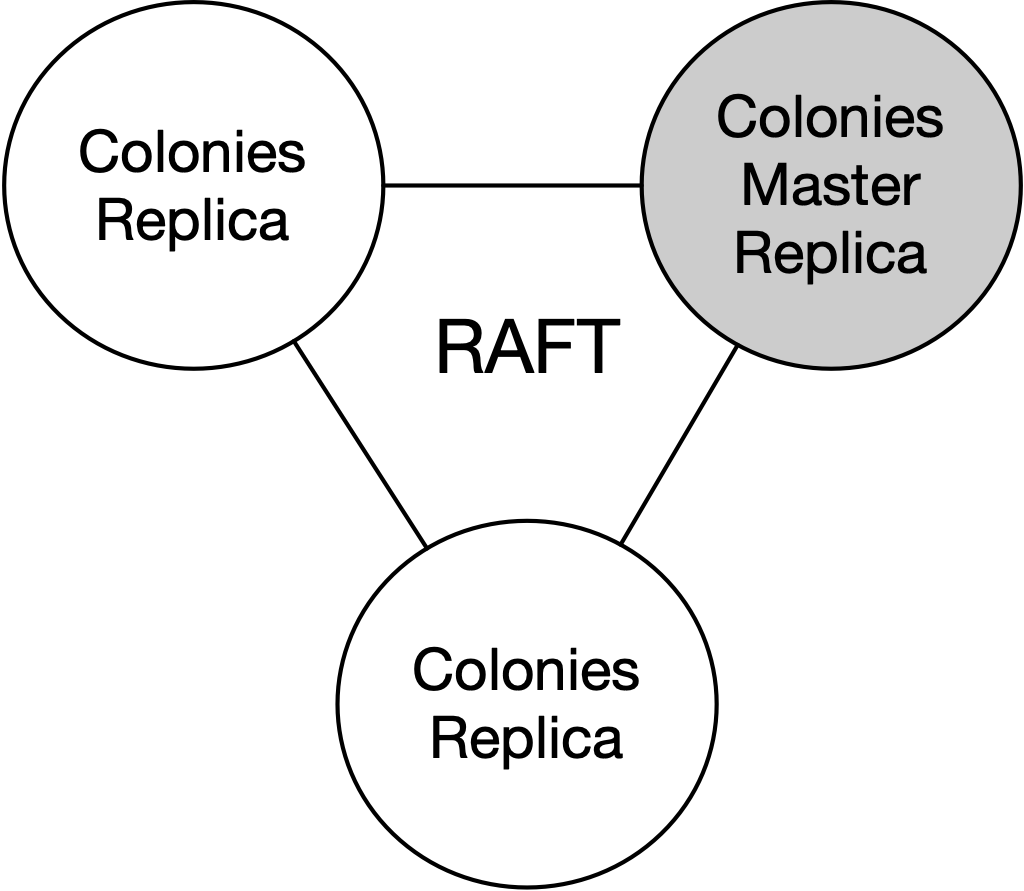
\includegraphics[scale=0.4]{raft.png}
	\caption{cron management}
	\label{fig:fig1}
\end{figure}

\subsubsection{Workflows}
TODO
\begin{figure}[h]
	\centering
    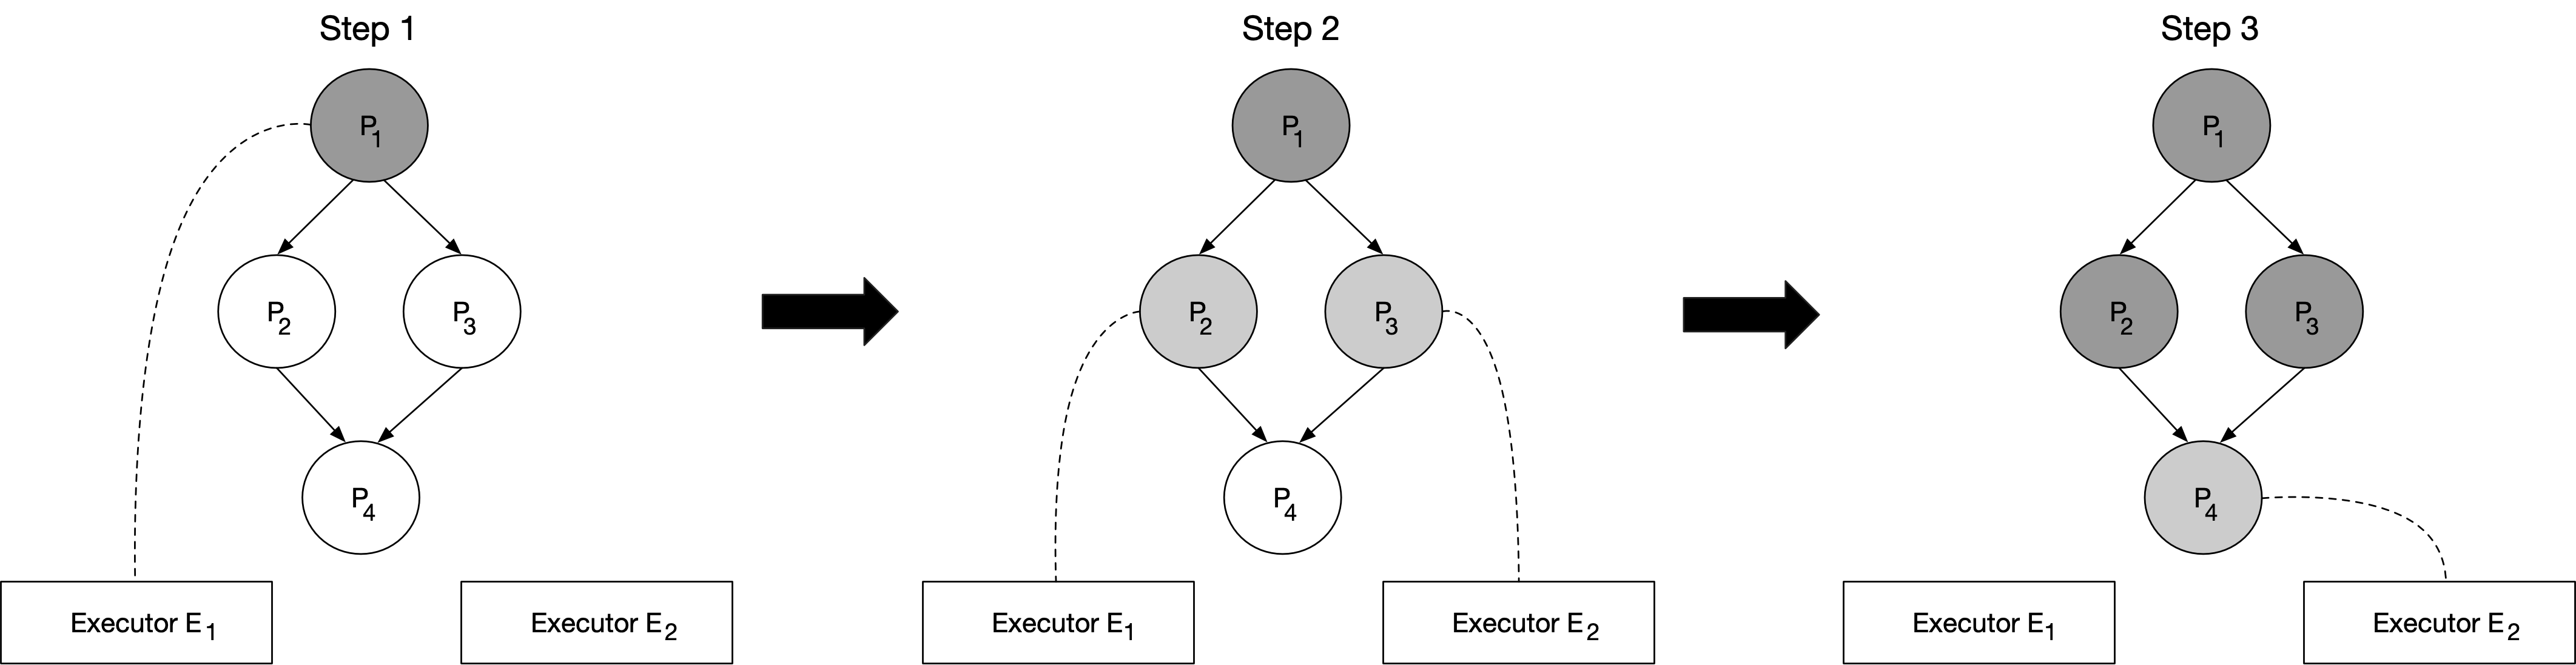
\includegraphics[scale=0.32]{workflow.png}
	\caption{cron management}
	\label{fig:fig1}
\end{figure}

\begin{table}[h]
	\caption{Function Specifications}
	\centering
	\begin{tabular}{llllll}
		\toprule
		\cmidrule(r){1-2}
        Function Spec & Function        & Executor Type & Priority & Max Exec Time & Max Retries \\
		\midrule
        $F_{1}$       & gen\_nums()     & Edge          & 1        & 200 s         & 5 \\
        $F_{2}$       & square()        & Cloud         & 1        & 200 s         & 5 \\
        $F_{3}$       & square()        & Cloud         & 1        & 200 s         & 5 \\
        $F_{4}$       & sum()           & Browser       & 1        & 200 s         & 5 \\
		\bottomrule
	\end{tabular}
	\label{tab:table}
\end{table}

\begin{table}[h]
	\caption{Snapshot of Process Table as in Step 2}
	\centering
	\begin{tabular}{llllll}
		\toprule
		\cmidrule(r){1-2}
        Process Id & Function Spec & Wait for Parents & Assigned Executor Id & State      & Priority Time \\
		\midrule
        $P_{1}$    & $F_{1}$       & $False$          & $E_{1}$              & Successful & 1679906715352024000 \\
        $P_{2}$    & $F_{2}$       & $False$          & $E_{1}$              & Running    & 1679906715353453000 \\
        $P_{3}$    & $F_{3}$       & $False$          & $E_{2}$              & Running    & 1679906715354286000 \\
        $P_{4}$    & $F_{4}$       & $True$           & -                    & Waiting    & 1679906715355188000 \\
		\bottomrule
	\end{tabular}
	\label{tab:table}
\end{table}

dt = -1000000000 * 60 * 60 * 24
process.PriorityTime = int64(process.FunctionSpec.Priority)*dt + submissionTime.UnixNano()


\begin{table}[h]
	\caption{Dependency Table}
	\centering
	\begin{tabular}{lll}
		\toprule
		\cmidrule(r){1-2}
        Process Id & Name       & Dependencies           \\
		\midrule
        $P_{1}$    & $Task_{1}$ & -                      \\
        $P_{2}$    & $Task_{2}$ & $Task_{1}$             \\
        $P_{3}$    & $Task_{3}$ & $Task_{1}$             \\
        $P_{4}$    & $Task_{4}$ & $Task_{2}$, $Task_{3}$ \\
		\bottomrule
	\end{tabular}
	\label{tab:table}
\end{table}
	
\begin{table}[h]
	\caption{Input/Output Table}
	\centering
	\begin{tabular}{lll}
		\toprule
		\cmidrule(r){1-2}
        Process Id & Input & Output \\
		\midrule
        $P_{1}$    & & [2,3] \\
        $P_{2}$    & 2 & 4 \\
        $P_{3}$    & 3 & 9 \\
        $P_{4}$    & [4,9] & 13 \\
		\bottomrule
	\end{tabular}
	\label{tab:table}
\end{table}

\subsubsection{Cron}
TODO
\begin{figure}[h]
	\centering
    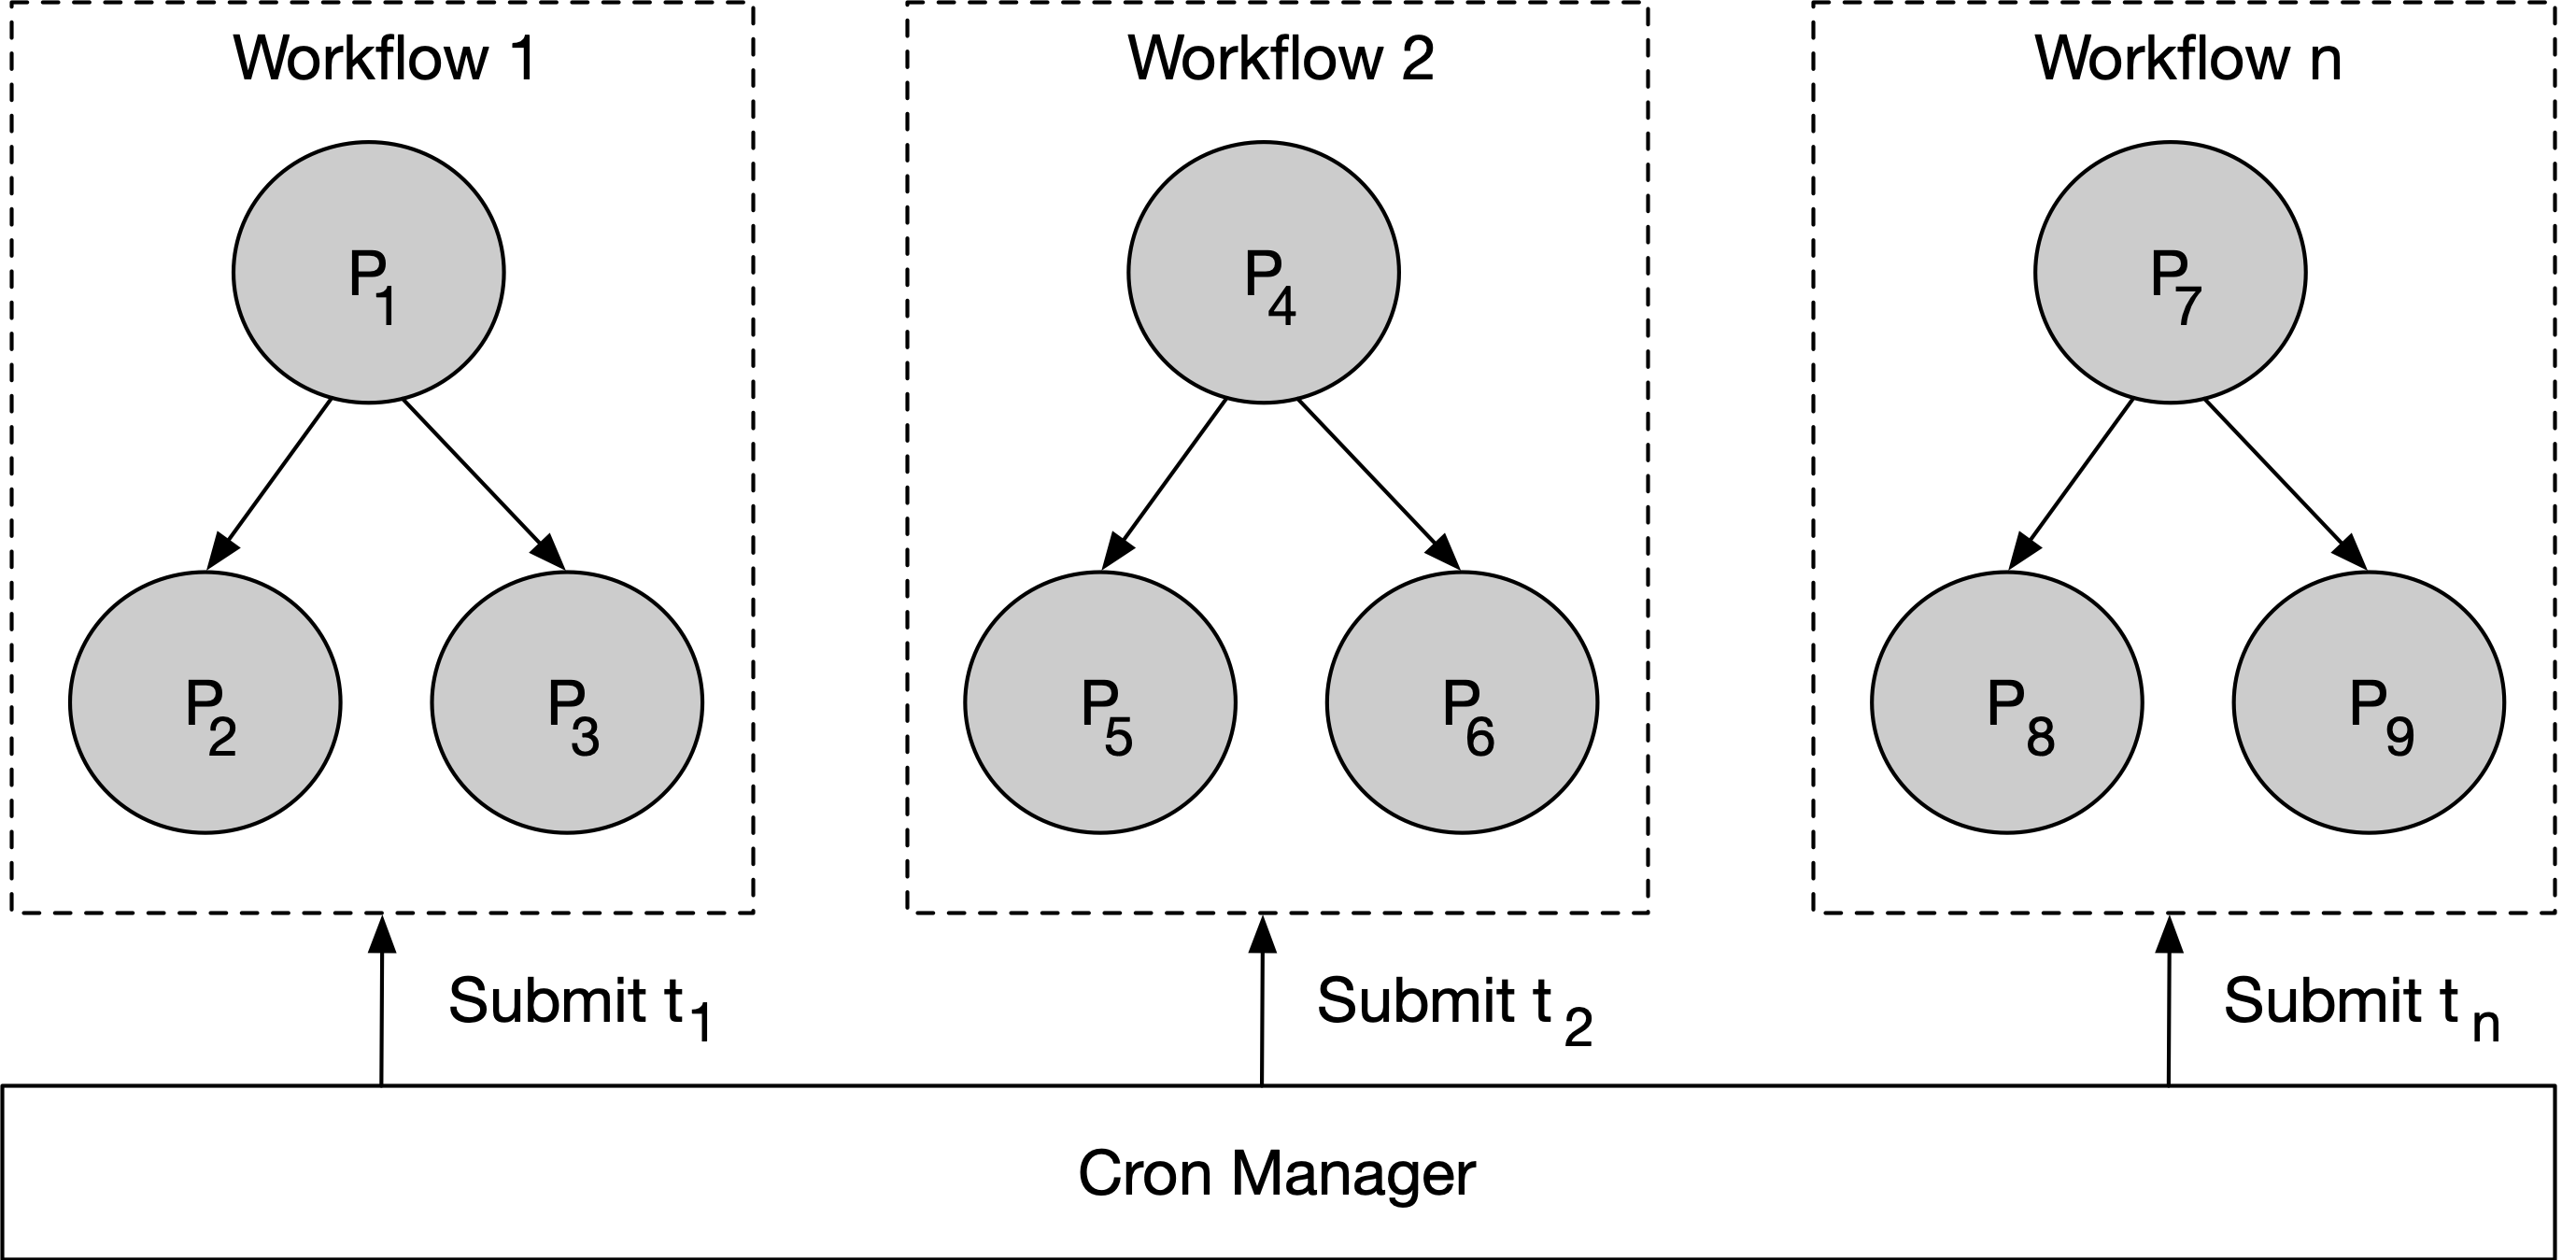
\includegraphics[scale=0.4]{cron.png}
	\caption{Sample figure caption.}
	\label{fig:fig1}
\end{figure}

\subsubsection{Generators}
TODO

\subsubsection{Zero-trust security}
TODO

\section{Evaluation}
\subsection{Implementation}
\begin{lstlisting}[language=c]
gen_nums = Function(gen_data, colonyid, executortype="edge")
square1 = Function(square, colonyid, executortype="cloud")
square2 = Function(square, colonyid, executortype="cloud")
sum = Function(square, colonyid, executortype="browser")

wf = ColoniesWorkflow("localhost", 50080, colonyid, executor_prvkey)
wf >> gennums
gennums >> square1
gennums >> square2
[square1, square2] >> sum
res = wf.execute()
\end{lstlisting}

\subsection{References}
TODO
\bibliographystyle{unsrtnat}
\bibliography{references}  %%% Uncomment this line and comment out the ``thebibliography'' section below to use the external .bib file (using bibtex) .


%%% Uncomment this section and comment out the \bibliography{references} line above to use inline references.
% \begin{thebibliography}{1}

% 	\bibitem{kour2014real}
% 	George Kour and Raid Saabne.
% 	\newblock Real-time segmentation of on-line handwritten arabic script.
% 	\newblock In {\em Frontiers in Handwriting Recognition (ICFHR), 2014 14th
% 			International Conference on}, pages 417--422. IEEE, 2014.

% 	\bibitem{kour2014fast}
% 	George Kour and Raid Saabne.
% 	\newblock Fast classification of handwritten on-line arabic characters.
% 	\newblock In {\em Soft Computing and Pattern Recognition (SoCPaR), 2014 6th
% 			International Conference of}, pages 312--318. IEEE, 2014.

% 	\bibitem{hadash2018estimate}
% 	Guy Hadash, Einat Kermany, Boaz Carmeli, Ofer Lavi, George Kour, and Alon
% 	Jacovi.
% 	\newblock Estimate and replace: A novel approach to integrating deep neural
% 	networks with existing applications.
% 	\newblock {\em arXiv preprint arXiv:1804.09028}, 2018.

% \end{thebibliography}

\end{document}
